\chapter{Tâche: Analyse de risques HAZOP}

\paragraph{Quels sont les dangers présentés par les substances mises en oeuvre durant la synthèse de l'ammoniac ?}
\begin{enumerate}
\item Azote : \ce{N2}
\begin{itemize}
\item Inodore et incolore
\item Risques de suffocation très rapide, donc dangereux dans des espaces confinés
\item Demande une grande quantité d’énergie pour être dissocié
\item À l'état liquide (sa température d'ébullition étant de $-196\,\celsius$), il peut provoquer des gelures, pouvant même être mortelles si elles ont lieu sur une grande surface de peau. Il peut également diminuer la résistance de certains matériaux qui peuvent alors se briser facilement.
\end{itemize}
\item Hydrogène : \ce{H2}
\begin{itemize}
\item Extrêmement explosif et inflammable : il réagit avec l'air, l'oxygène ou encore des halogènes.
\item Conséquences après inhalation de grosses concentrations : maux de tête, sifflements dans les oreilles, vertiges, pertes de connaissance, somnolences,  nausées, vomissements, etc.
\item Extrêmement volatile (même à travers certains métaux, donc problème de matériaux)
\item Problèmes de corrosion dans les réacteurs, dus à la réaction
\ce{Fe3C + 2H2 -> CH4 + 3Fe}.
Cette réaction produit du fer pur, ce qui va introduire de la rouille dans le réacteur.
\end{itemize}
\item Ammoniac : NH$_3$
\begin{itemize}
\item À une concentration de $700\,\milli\gram\per\meter\cubed$, effets irréversibles après 3 minutes
\item Lorsque l'ammoniac est dissous dans l'eau, il forme de l'hydroxyde d'ammonium (\ce{NH4+} et \ce{OH-}), connu sous le nom d'\emph{ammoniaque}. L'inhalation d'ammoniaque, son ingestion ou un contact direct avec la peau peuvent causer des difficultés pour respirer, des douleurs dans la gorge, des brûlures, des irritations, etc.
\item Incolore mais très odorant
\item Plus léger que l’air
\item Température critique élevée ($132.4\,\celsius$), donc facile à liquéfier
\item Stable à température normale
\item Explosif en présence d’air
\item Réagit très rapidement avec l’eau
\item Extrêmement polluant
\end{itemize}
\end{enumerate}

\quest{Comment les flux de matière circulent-ils dans la section indiquée et au sein du réacteur de conversion ?}
Ces flux ont été surlignés dans les figures \ref{ann2}, \ref{ann3} et \ref{ann4}. On a utilisé différentes couleurs pour montrer les liens entre les flux des différentes fiches.


\begin{figure}
\centering
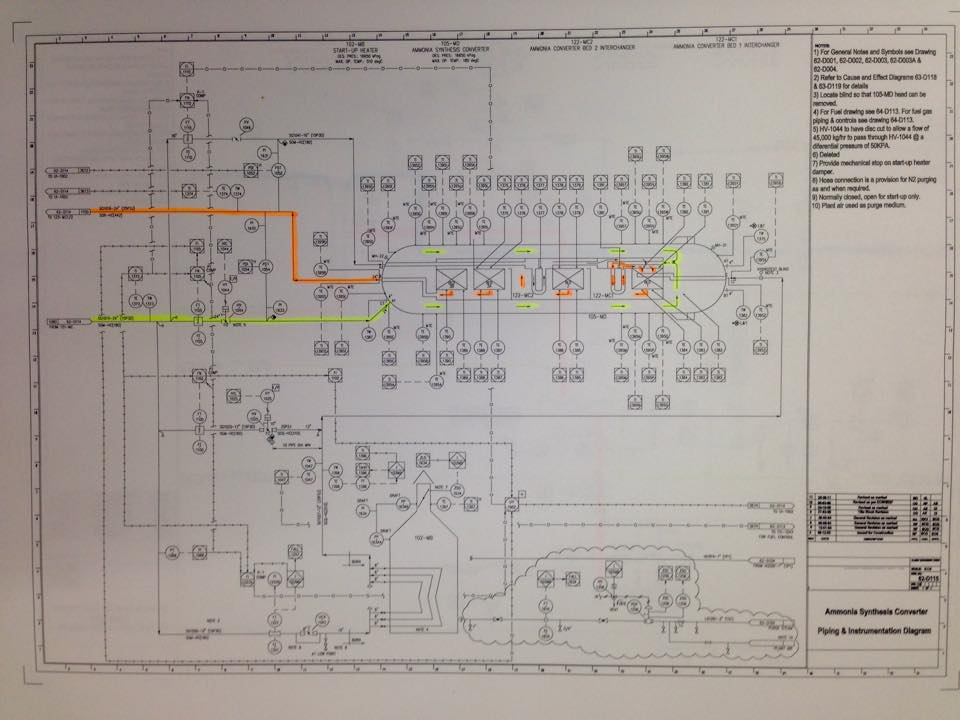
\includegraphics[width=0.8\textwidth]{img/hazop1}
\caption{PID du réacteur de synthèse}
\label{ann2}
\end{figure}

\begin{figure}
\centering
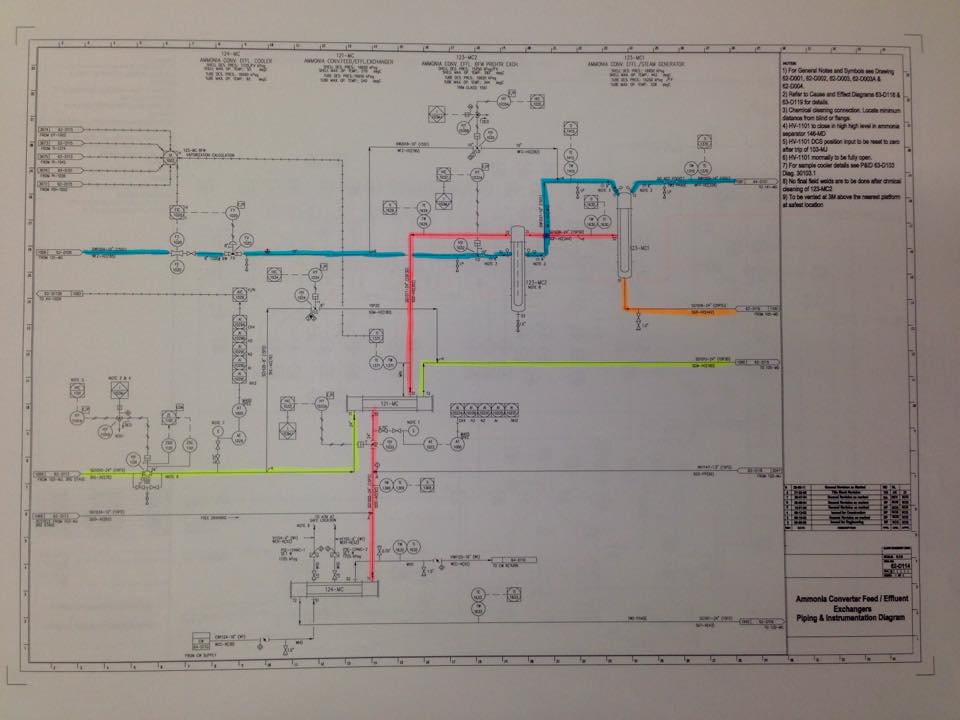
\includegraphics[width=0.8\textwidth]{img/hazop2}
\caption{PID des échangeurs}
\label{ann3}
\end{figure}

\begin{figure}
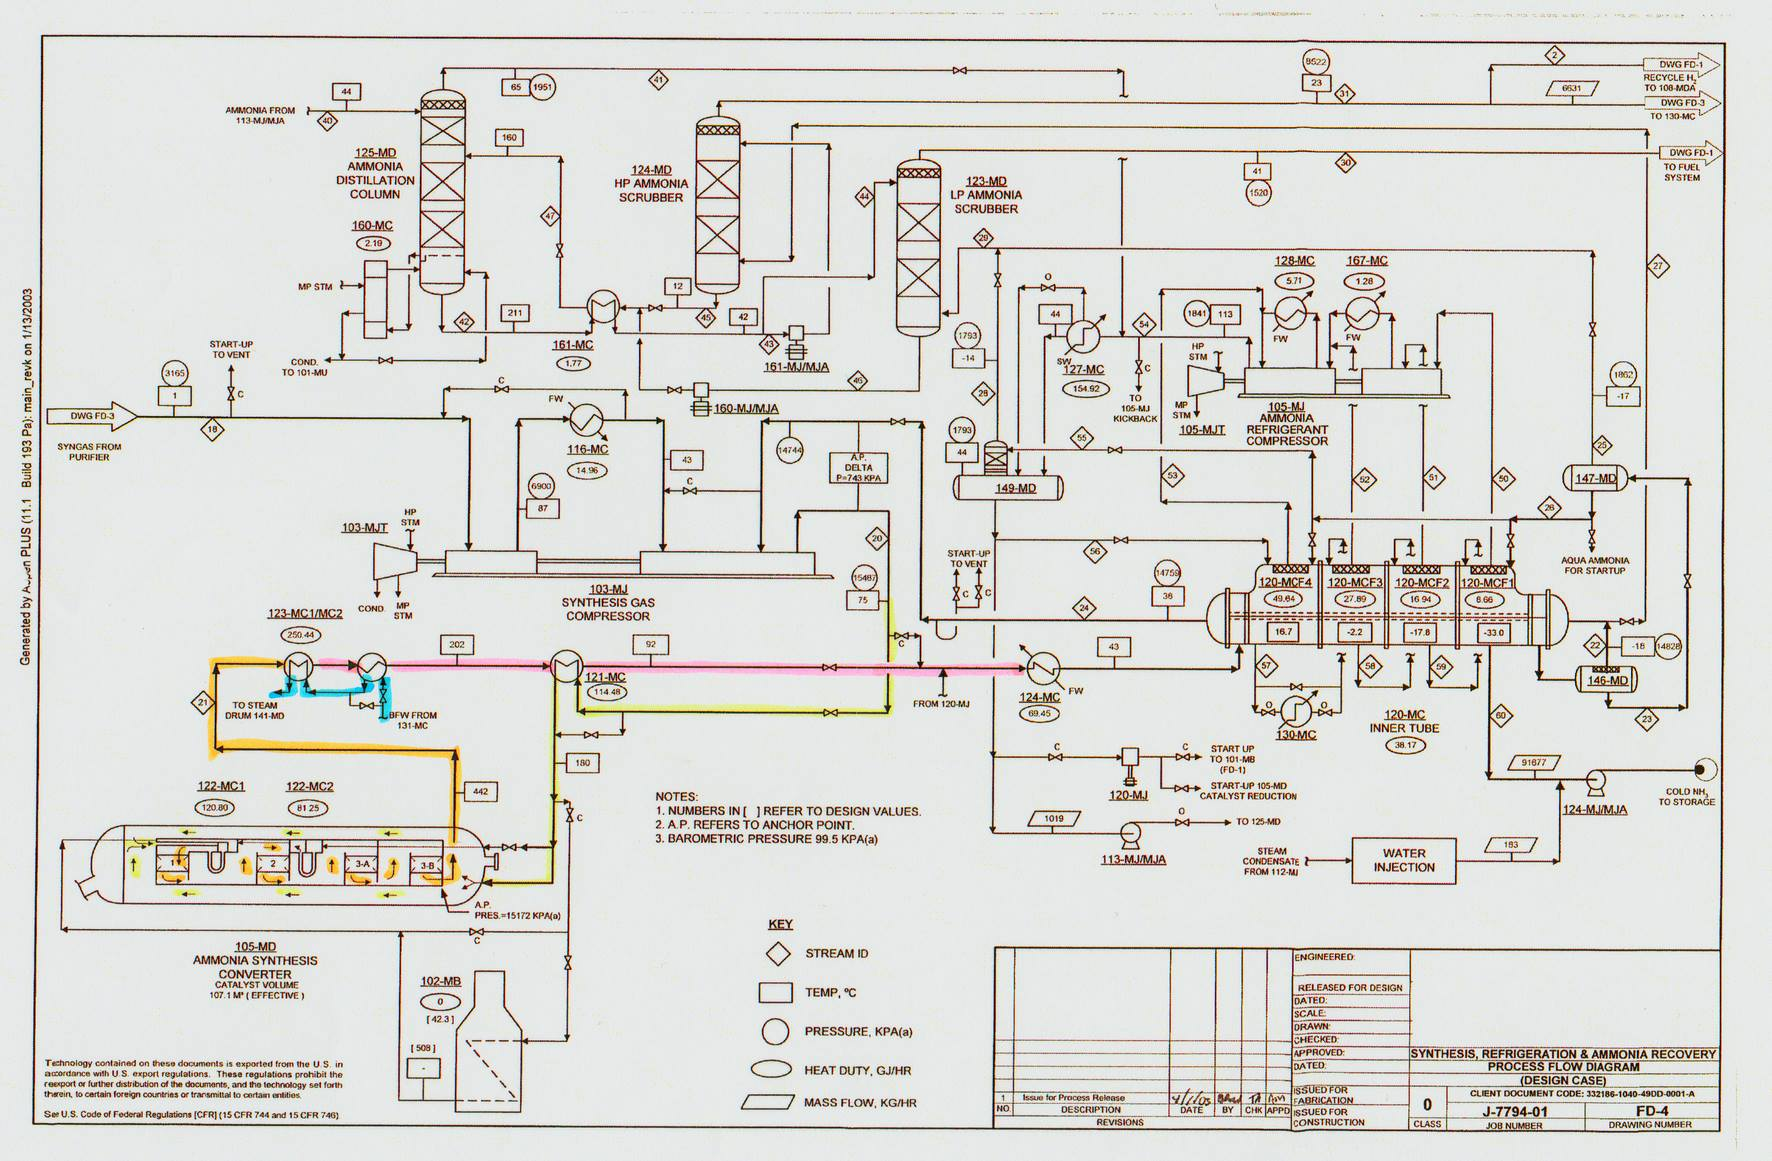
\includegraphics[width=\textwidth]{img/hazop3}
\caption{PFD du système de synthèse complet}
\label{ann4}
\end{figure}

\quest{Imaginez 3-4 scénarios (déviation-causes-conséquences) et suggérez des barrières pour chacun d'eux}
Nos scénarios sont présentés dans la table~\ref{scenarii}.

\begin{table}
\centering
\footnotesize{
\begin{tabular}{|p{0.12\textwidth}|p{0.15\textwidth}|p{0.35\textwidth}|p{0.26\textwidth}|}
\hline
\textbf{Déviation} & \textbf{Cause(s)} & \textbf{Conséquence(s)} & \textbf{Mesure(s) de maîtrise} \\ \hline \hline
\textbf{1} Eau	dans le tuyau & \textbf{1.1} Fuite dans le refroidisseur 123-MC2 & \textbf{1.1.A}	Refroidissement des vapeurs

\textbf{1.1.B}	Baisse	de la pression

\textbf{1.1.C}	Contaminant	(eau)	dans	les	
produits

\textbf{1.1.D}	 Pas de conséquences en terme de sécurité &
\textbf{1.1.C.a} Prévoir une redirection du flux vers un système de condensation de l’eau afin d’éliminer le contaminant	\\ \hline

\textbf{2} Augmentation de la température & \textbf{2.1} L’eau ne circule plus dans le système de refroidissement 131-MC (pour	cause	de gel) &
\textbf{2.1.A}	Flux d’entrée du réacteur trop réchauffé ce qui défavorise l’équilibre

\textbf{2.1.B}	Reste	trop de moles de \ce{N2} et de \ce{H2} $\rightarrow$ Augmentation de la pression mais régulation par le compresseur prévue

\textbf{2.1.C}	Pas de conséquences en terme de sécurité	
&
\textbf{2.1.A.a} Mettre de l’antigel dans le système de refroidissement \\ \hline
\textbf{3} Pas	de flux & \textbf{3.1} Fermeture erronnée de la vanne entre le 121-MC et 124-MC &
\textbf{3.1.A}	Stagnation des vapeurs dans les refroidisseurs en amont, 123-MC1 et 2, qui continuent à tourner.	
Le gaz se refroidit donc juqu’à atteindre la température de l’eau.

\textbf{3.1.B}	Risque d’endommagement mécanique de l’échangeur à cause du changement de température

\textbf{3.1.C}	Risque de fuites de produits dans l’échangeur &
\textbf{3.1.A.a} Contrôle automatique de la vanne via un thermomètre au niveau de l’échangeur de chaleur 123-MC2

\textbf{3.1.C.a} Système d’aspiration des vapeurs échappées

\textbf{3.1.C.b} Enveloppe de protection autour du tuyau\\ \hline

\end{tabular}
}
\caption{Scénarios possibles pour le tuyau entre les échangeurs de chaleur 123-MC2 et 121-MC}
\label{scenarii}
\end{table}

\quest{Pourquoi n'y a-t-il pas de soupape de sécurité ou de disque de rupture sur le réacteur de synthèse du \ce{NH3} ?}
Un disque de rupture est un dispositif de sécurité qui sert à protéger les installations contre les risques de variation de pression, et son fonctionnement repose sur une membrane étanche qui se rompt lorsque la pression de rupture est atteinte. \cite{disque}
Comme une pression constante ($p=15\,172\,\kilo\pascal$) est assurée au niveau du réacteur par le convertisseur, il n'y a a priori pas de risque de surpression, et donc pas besoin de soupape de sécurité ou de disque de rupture.
De plus, le nombre de moles de gaz dans les produits est plus petit que celui dans les réactifs, et donc, si la réaction s'emballe, la pression diminue.

\quest{Pourquoi y a-t-il des disques de rupture sur l'échangeur 124-MC ?}
Si l'échangeur avait un dysfonctionnement,
et refroidissait moins bien voire pas du tout le flux qui passe à travers,
cela augmenterait la température et causerait donc une surpression.
Par conséquent, il faut des disques de rupture pour gérer cet incident
rare mais possible.
